\section{Development Models and Separate Comparisons}
\label{app:development-results}
These experiments concern the original pooled-source controller and a separately selected Jinan model. Each comparison retains its own fitted controller, target data, and evaluation protocol. The final frozen source-selector comparison is reported in Section~\ref{sec:results}.

\subsection{Offline phase selection}
In the seven development groups, mean normalized regret decreases from 0.24142 for the restricted reference predictor to 0.21767 for the selected blend, a reduction of 9.84\%. Six groups improve. Hangzhou worsens by 0.00388, showing that the average improvement does not hold uniformly across groups. These results concern the development adaptation exercises, not seven independent external cities.

The external offline test is summarized in Table~\ref{tab:offline}. Equal-city regret decreases from 0.29219 to 0.26854, an 8.09\% reduction. Los Angeles improves by 2.18\%, but its paired improvement interval crosses zero. Jinan improves by 10.10\%, with a positive group-bootstrap improvement interval. Correct selection of the minimum-cost action increases from 78.5\% to 81.0\% in Los Angeles and from 29.6\% to 34.2\% in Jinan. The unequal accuracies also indicate that the two targets differ substantially in ranking difficulty.

\begin{table}[!t]
\caption{Original Pooled-Source Controller: External Offline Regret}
\label{tab:offline}
\centering
\begin{tabular}{lrrr}
\toprule
Target & Reference & Original \method & Reduction\\
\midrule
Los Angeles & 0.14824 & 0.14501 & 2.18\%\\
Jinan & 0.43615 & 0.39208 & 10.10\%\\
Equal-city mean & 0.29219 & 0.26854 & 8.09\%\\
\bottomrule
\end{tabular}
\vspace{3pt}
\begin{minipage}{\columnwidth}\footnotesize
Lower regret is better. Paired 95\% intervals for absolute regret reduction are $[-0.06747,0.07289]$ for Los Angeles and $[0.00469,0.08293]$ for Jinan. Test groups come from one held-out seed.
\end{minipage}
\end{table}

\subsection{Initial comparison of the original controller}
Table~\ref{tab:closedloop} reports all seven controllers. The original controller achieves 149.17~s mean waiting, compared with 159.15~s for the dense linear residual model. The reduction is 9.98~s, or 6.27\%, with a paired bootstrap interval of $[2.01,17.19]$~s. Waiting decreases in both targets: by 8.46~s in Los Angeles and 11.50~s in Jinan. Completed-trip waiting and system vehicle-hours also decrease in this comparison.

\begin{table*}[!t]
\caption{Original Controller: Initial Outcomes Over Four Scenarios and Two Seeds}
\label{tab:closedloop}
\centering
\begin{tabular}{lrrrrrr}
\toprule
& \multicolumn{3}{c}{Waiting, all departed vehicles (s)} & Completed-trip & System & Demand\\
\cmidrule(lr){2-4}
Controller & Los Angeles & Jinan & Equal-city mean & waiting (s) & vehicle-hours & completion\\
\midrule
Fixed time & 507.33 & 169.84 & 338.58 & 308.72 & 885.18 & 0.661\\
Dense linear residual & 212.88 & 105.41 & 159.15 & 147.47 & 618.15 & 0.870\\
Simulator prior & 219.17 & 94.26 & 156.71 & 138.68 & 619.66 & 0.877\\
Reference predictor & 206.78 & 99.05 & 152.91 & 138.40 & 606.30 & 0.882\\
\method, original & 204.42 & 93.91 & 149.17 & 133.06 & 594.14 & 0.889\\
PhasePressure & 197.51 & \textbf{89.73} & 143.62 & \textbf{125.32} & 583.05 & \textbf{0.898}\\
MaxPressure & \textbf{191.89} & 91.58 & \textbf{141.74} & 135.42 & \textbf{580.29} & 0.896\\
\bottomrule
\end{tabular}
\end{table*}

Relative to the simulator prior and reference predictor, the proposed controller reduces the waiting point estimate by 4.81\% and 2.45\%, respectively. Their intervals cross zero. Thus, the initial closed-loop evidence is clearest for the comparison with the dense linear residual. Since both methods use matched action differences, that gain cannot be credited to reference subtraction alone. The different regressors and weighting procedures also prevent an isolated claim about causal feature restrictions.

The two pressure controllers achieve the lowest equal-city waiting times in this initial comparison. MaxPressure outperforms the original \method\ by 7.43~s and PhasePressure by 5.55~s. Both also reduce system vehicle-hours and improve completion. Their superiority is visible in each target, so it is not an artifact of averaging a Los Angeles gain against a Jinan loss.

All 56 runs complete without teleports. The eight proposed-controller runs contain no consolidated junction-collision incidents. This small initial sample is insufficient to establish a safety advantage, especially given the larger comparison below.

\subsection{Independent confirmation with frozen models}
We evaluate the same proposed and dense linear residual models on ten new paired seeds across the original four scenarios. All 80 runs complete without refitting or parameter tuning. Equal-city waiting decreases from 158.67 to 150.84~s, a reduction of 7.83~s or 4.93\% (Table~\ref{tab:dense-confirmation}). The paired 95\% interval is 4.11--11.85~s for the absolute reduction and 2.64--7.31\% for the relative reduction. The prespecified confirmation criterion is met, and nine of ten equal-city seed means improve. Los Angeles improves by 5.43~s on average, with six favorable seeds; Jinan improves by 10.22~s, with all ten favorable (Fig.~\ref{fig:dense-confirmation}). Completed-trip waiting decreases from 147.49 to 132.88~s, system vehicle-hours from 616.49 to 596.15, and completion increases from 87.59\% to 88.66\%. All runs have zero teleports. These results confirm the frozen controller's advantage over the tested linear residual baseline on new seeds of the same networks.

\begin{table}[!t]
\caption{Original Pooled-Source Controller: Ten-Seed Confirmation}
\label{tab:dense-confirmation}
\centering
\begin{tabular}{lrrrr}
\toprule
& \multicolumn{2}{c}{Waiting (s)} & & \\
\cmidrule(lr){2-3}
Target & Dense & Original & Reduction & Improved\\
\midrule
Los Angeles & 213.07 & 207.64 & 2.55\% & 6/10\\
Jinan & 104.27 & 94.05 & 9.80\% & 10/10\\
Equal-city mean & 158.67 & 150.84 & 4.93\% & 9/10\\
\bottomrule
\end{tabular}
\vspace{3pt}
\begin{minipage}{\columnwidth}\footnotesize
Waiting includes unfinished trips. Jinan demands and then cities are weighted equally. The overall relative reduction is computed from the two macro means, with a paired 95\% interval of 2.64--7.31\%. Improved counts refer to seed-level waiting means.
\end{minipage}
\end{table}

\begin{figure*}[!t]
\centering
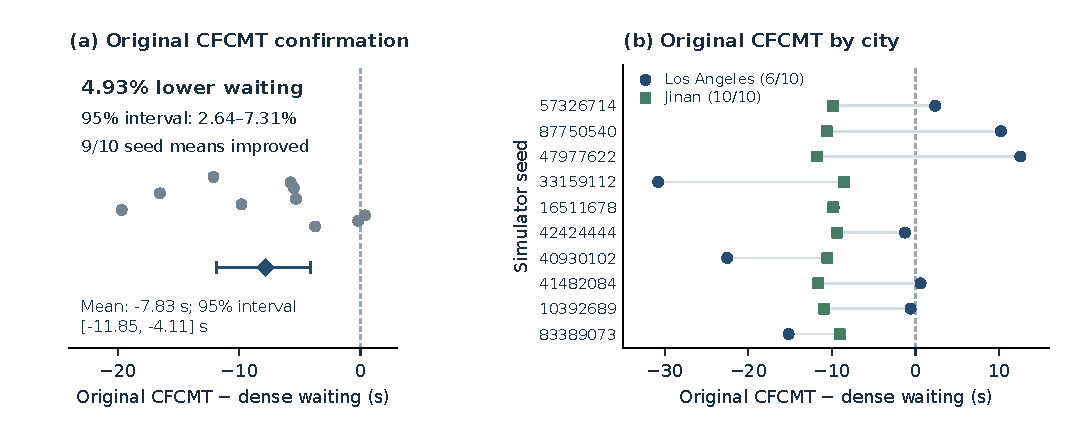
\includegraphics[width=\textwidth]{fresh_seed_confirmation.pdf}
\caption{Original pooled-source controller: frozen-model confirmation on ten new paired seeds. (a) Grey points show equal-city waiting differences for all ten seeds, with vertical offsets for visibility; the diamond shows the overall mean with its registered 95\% interval from 20,000 paired seed-block bootstrap replicates. (b) City-specific differences retain the same seed pairing. Negative values favor the original \method. The interval describes seed variation within the two fixed target networks.}
\label{fig:dense-confirmation}
\end{figure*}

\subsection{Fresh seeds reveal different transfer outcomes}
The original seven-controller comparison did not include the existing target-dominated model as a closed-loop baseline. Adding that model afterwards to the original eight scenario--seed cells gives 149.04~s mean waiting, almost identical to \method's 149.17~s. Because the addition followed inspection of the main results, this comparison is descriptive.

We subsequently compare the unchanged controllers on 64 fresh seeds, one Los Angeles scenario and three Jinan scenarios, for 512 runs. The comparison model's deployed prediction weight is numerically entirely on target data, but a retained source prior can resolve exact score ties. We therefore call it the \emph{target-dominated comparator}, not a strictly source-free model. Both controllers use the same target adaptation groups and execution rules.

The equal-city mean waiting is 155.14~s for \method\ and 149.09~s for the comparator. The prespecified mean seed-level relative change in \eqref{eq:relative} is $+4.25\%$, with interval $[-0.77,13.21]\%$. Only 29 of 64 seed means improve. The city effects have opposite signs: Jinan improves by 3.04\%, with all 64 seed means favorable, while Los Angeles worsens by 7.87\%, with 22 favorable seeds.

The largest Los Angeles failure increases waiting from 194.74 to 975.27~s and reduces completion from 0.919 to 0.270. It has neither a teleport nor a collision and remains in the analysis. Across the full comparison, collision incidents total 25 for \method\ and 15 for the comparator. The prespecified requirement for joint benefit---including nonpositive average and interval upper bound, no city regression, at most 5\% worst-seed regression, and no excess incidents---is not met. More repetitions therefore do not confirm a general benefit from the original source-aware controller.

\subsection{A separately selected Jinan controller}
Following that result, a subsequent experiment refits the models and selects among seven source groups using only target action labels. It corrects static network context by tracing controlled movements through intermediate road links to the nearest downstream signals, then recomputes context-dependent analytic priors. Recorded action features and outcome labels are unchanged. Five folds, blocked by scenario and seed, evaluate a balanced set of 100 target action groups and source weights $\{0,0.25,0.5,0.75,1\}$. A source is used only if mean regret improves by more than 0.5\%, its one-sided 95\% upper bound for change is below zero, and no fold worsens by 1\% or more. Otherwise the procedure returns the target-only model. Before its new evaluation runs, it selects no source for Los Angeles and the Hangzhou component at weight one for Jinan.

On 56 further Jinan seeds and three demand scenarios, the selected controller reduces waiting by 4.53\%, with paired interval $[4.28,4.79]\%$; all 56 seed means improve. The experiment comprises 336 runs. This is a repeatable improvement over a lower-capacity model fitted only on target examples. Both arms use the same pressure-reference guard: a proposed phase can replace the reference only when its predicted cost contrast plus 0.5 times its error score is negative and its normalized pressure deficit is at most one. Otherwise, the reference phase is used. The deficit is $\max\{\Pi(r_g)-\Pi(a),0\}/\max\{|\Pi(r_g)|,1\}$, where $\Pi$ is the generalized-pressure score and $r_g$ is its reference phase in the current state. The multiplier 0.5 is inherited from earlier development. This comparison cannot separate the value of source data from the model change and cannot be pooled with the original controller's results. Table~\ref{tab:fresh} summarizes these two protocols.

\begin{table}[!t]
\caption{Fresh-Seed Comparisons Under Separate Protocols}
\label{tab:fresh}
\centering
\begin{tabular}{lrrr}
\toprule
Controller and target & Seeds & Change & Improved\\
\midrule
Original, two-city mean & 64 & $+4.25\%$ & 29/64\\
Original, Los Angeles & 64 & $+7.87\%$ & 22/64\\
Original, Jinan & 64 & $-3.04\%$ & 64/64\\
Revised controller, Jinan & 56 & $-4.53\%$ & 56/56\\
\bottomrule
\end{tabular}
\vspace{3pt}
\begin{minipage}{\columnwidth}\footnotesize
Negative change means lower waiting. The original controller is compared with the target-dominated model; the revised controller uses a smaller, strictly target-only comparator. The primary 95\% intervals are $[-0.77,13.21]\%$ for the two-city mean and $[-4.79,-4.28]\%$ for the revised controller. The rows are not estimates for one unchanged method.
\end{minipage}
\end{table}

\subsection{Additional development diagnostics}
The pressure comparisons keep this limitation visible. A separate later experiment using a 120-s predictor and a rate-limited executor also fails to establish an advantage over PhasePressure on 64 fresh Jinan seeds: its relative waiting change is $-0.043\%$, with interval $[-0.449,0.370]\%$. That controller differs from \method\ and is not an additional row in Table~\ref{tab:closedloop}. Further source-selection experiments on the seven development groups either retain harmful group-level effects or return target-only predictions. They provide no basis for replacing the negative cross-network result with a general transfer claim.


\subsection{Uncertainty for development comparisons}
Offline regret follows \eqref{eq:regret}. Group-level uncertainty uses 10,000 paired bootstrap replicates. For the initial closed-loop comparison, scenarios and seeds are paired between controllers. The 10,000-replicate hierarchical bootstrap resamples cities, then scenarios, then seeds. With only two target networks and two seeds per scenario, these intervals describe the observed experiment; they do not establish performance over a population of cities.

For the independent dense-baseline confirmation, ten new seeds are fixed before execution, excluding previously used and reserved seeds. Both models, network inputs, signal executor, and timing remain unchanged, giving 80 runs on the original four scenarios. No refitting, new target labels, or parameter tuning is used. Within each seed, the three Jinan demands are averaged equally, followed by equal city weights and then equal weights across seeds. The primary effect is the difference between the two overall waiting means; relative change divides this difference by the dense mean. It is not the mean of seed-level percentages. The 95\% percentile interval uses 20,000 paired bootstrap replicates with NumPy PCG64, initialized with 20261022. Each replicate resamples ten complete seed blocks, keeping both controllers and all four scenarios together. Cities are not resampled. Confirmation requires all 80 valid records, a negative mean waiting difference, and a negative upper interval endpoint. All ten seeds are retained, and these runs are not pooled with the other experiments.

In the 64-seed target-dominated comparison, each seed $k=1,\ldots,N$, with $N=64$, produces an equal-scenario mean for each city and then an equal-city mean $\overline W_k^\pi$ for controller $\pi$. Relative change is
\begin{equation}
 \rho_k=\frac{\overline W_k^{\mathrm{proposed}}-
 \overline W_k^{\mathrm{comparison}}}{\overline W_k^{\mathrm{comparison}}},
 \qquad \overline\rho=\frac{1}{N}\sum_{k=1}^{N}\rho_k.
 \label{eq:relative}
\end{equation}
Negative values indicate lower waiting. The mean of these ratios is distinct from the ratio of the two pooled waiting means. Fresh-seed intervals resample complete paired seeds. No adverse evaluation seed is removed.

\subsection{Original local blending rule}
Candidate combinations include constant choices $\alpha_g\in\{0,0.1,\ldots,1\}$ shared across groups, and a local rule that limits departures from $A_g$.

Let $a_A$ and $a_P$ minimize $A_g$ and $P_g$, respectively, and write $\range(v)=\max_av(a)-\min_av(a)$. The rule computes
\begin{align}
 h_g&=\max\{\range(A_g),\median_a u_{A,g}(a),10^{-6}\},\nonumber\\
 D_g&=\range(P_g-A_g)/h_g,\nonumber\\
 M_g&=\{P_g(a_A)-P_g(a_P)\}/h_g,\nonumber\\
 U_g&=\{u_{P,g}(a_A)+u_{P,g}(a_P)\}/h_g,\nonumber\\
 \alpha_g&=\min\{1,\kappa/\max(D_g,10^{-12})\}
 \ind\{M_g\geq\zeta U_g\}.
 \label{eq:localblend}
\end{align}
The scale $h_g$ normalizes model disagreement $D_g$, the pairwise margin $M_g$, and the combined error score $U_g$; $\ind\{\cdot\}$ equals one when its condition holds and zero otherwise. The cap $\kappa\in\{0.25,0.5,1,2,4\}$ and error multiplier $\zeta\in\{0,0.25,0.5,1\}$ are selected on target validation data. If the indicator fails, the pooled-source predictor uses $A_g$. Otherwise,
\begin{equation}
 \range(S_g-A_g)=\alpha_g\range(P_g-A_g)\leq\kappa h_g.
 \label{eq:cap}
\end{equation}

\emph{Score-cap derivation.}
To verify \eqref{eq:cap}, note that $S_g-A_g=\alpha_g(P_g-A_g)$ and $\alpha_g\geq0$,
\begin{equation*}
 \range(S_g-A_g)=\alpha_g h_gD_g\leq\kappa h_g,
\end{equation*}
where the last step follows from \eqref{eq:localblend}, including $D_g=0$.

\subsection{Original pooled-source blend selection}
In the original blend-selection procedure, two target simulation seeds supply adaptation groups. In each validation fold, both predictors are fitted on all source examples and one target seed, then evaluated on the other target seed. Regret is first averaged over groups within each demand scenario, then equally over scenarios and the two folds. A candidate blend must not worsen mean validation regret relative to $A_g$, and its regret increase in either complete-seed fold must be at most 0.1. Among admissible candidates, we select the one with lowest mean regret, using deterministic tie breaking. The pure reference predictor remains available. Los Angeles selects $(\kappa,\zeta)=(1,0.25)$, while Jinan selects constant $\alpha_g=0.9$.

After selection, both predictors are fitted again on the source data and all target adaptation groups. The fold-specific models are discarded. Online control extracts traffic features, scores every feasible phase with \eqref{eq:blend}, and passes the minimizing phase to the common executor. There is no online retraining, simulator branching, or uncertainty-based guard in this original controller. Sparse coordination still returns the pressure reference for blocked proposals. The pressure reference is still computed to define the score origin.

